% An open problem is the visualization of real-time vehicles data. The problem relies on the fact that most of todays transit APIs will update bus positions about every minute, and therefore some interpolation is needed to animate vehicles on a map. A very rough approach is to update bus position only when there is a new update, but this cause the vehicle to jump from the old position to the new position and makes it difficult to estimate vehicles movement directions; moreover, the vehicle position is out of date until a new update comes. Although a higher frequency for position updates seems desirable it would also increase the battery consumption on your mobile phone querying the requests while also increase the server load that needs to process it. New visualizations should study how to effectively interpolate bus updates, which is not an easy to solve problem. 
  % [see transit_state_of_the_art.pdf P. 8 section 6.4]
  
\subsection{Probleme und Herausforderungen}
\label{sub:probleme_und_herausforderungen}

  Die Visualisierung von Echtzeitdaten bringt einige Schwierigkeiten und Herausforderungen mit sich. Diese werden in diesem Abschnitt gesammelt und beschrieben.

  \subsubsection{Bewältigung der Datenmenge}
  \label{ssub:bewältigung_der_datenmenge}
    An einem Montag den 28.08.2017 zwischen 3.00 und 24.00 Uhr zeigt Abbildung \ref{fig:activeTrips}: Nach einem rapiden Anstieg in der Morgenzeit, erreicht die Anzahl an aktiven Trips ihre Maxima um 07.04 mit 779. 

    \begin{figure}[ht]
      \begin{center}
        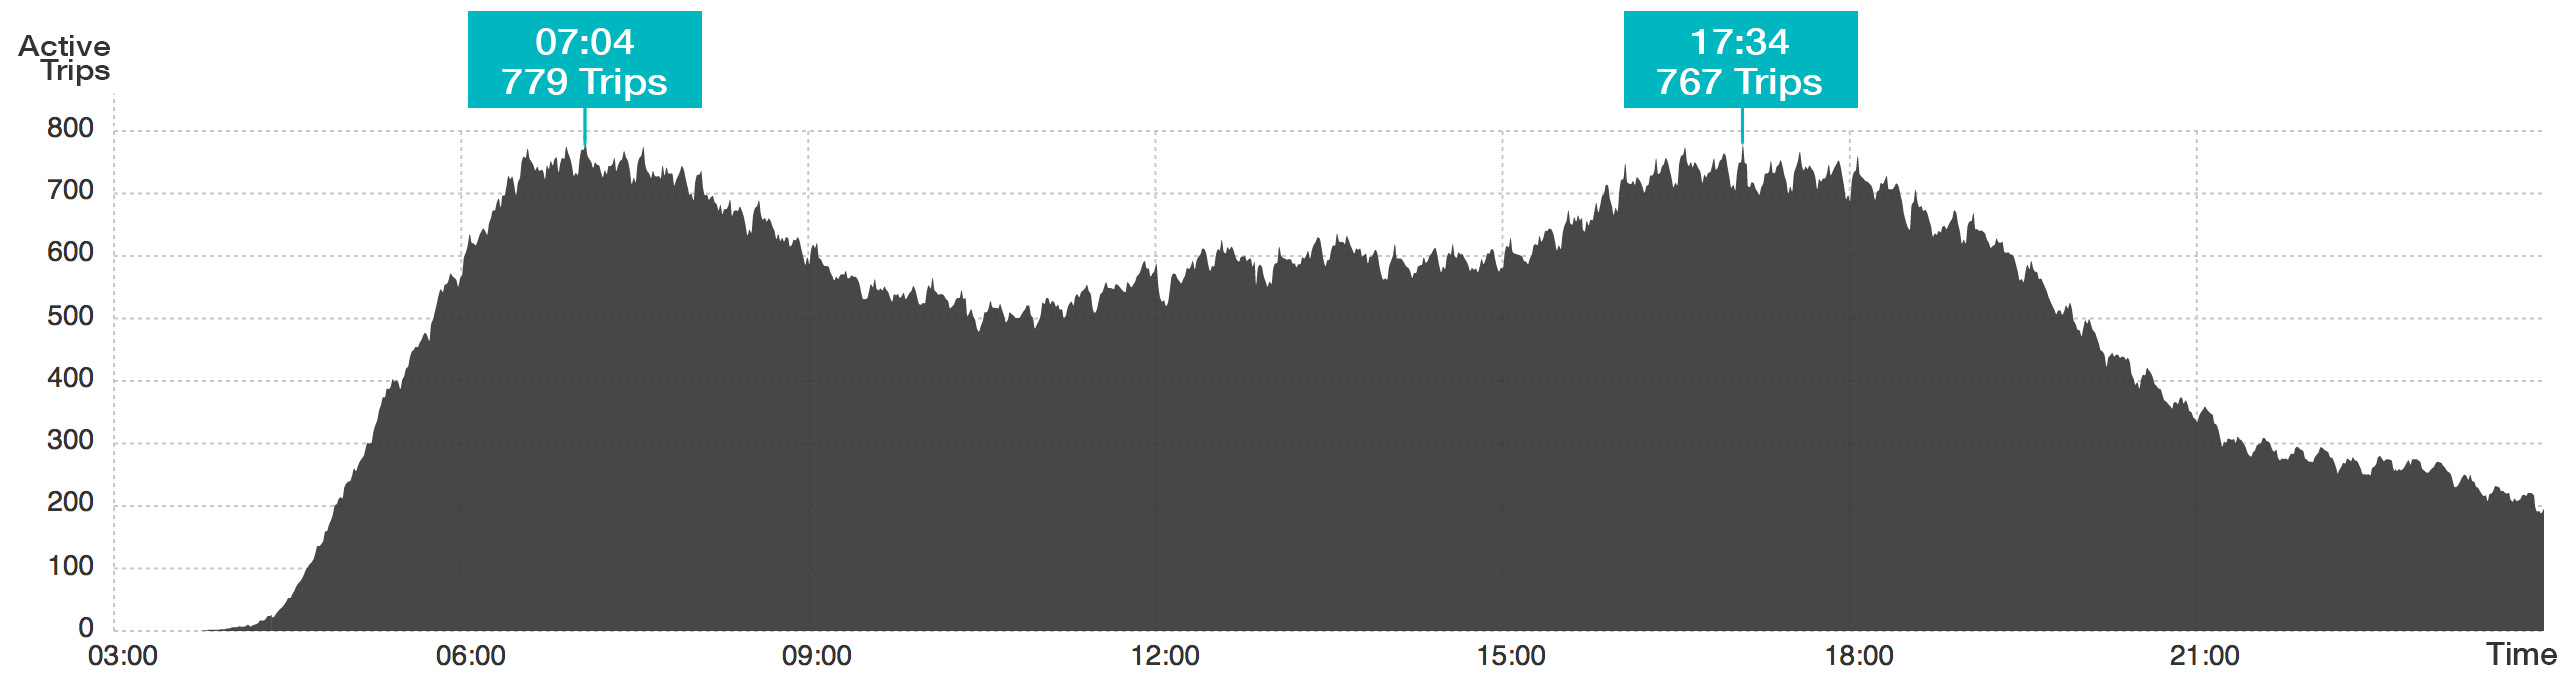
\includegraphics[width=\textwidth]{activeTrips.jpg}
        \caption{Anzahl an aktiven Trips zwischen 3.00 und 24.00 Uhr am 02.08.2017}
        \label{fig:activeTrips}
      \end{center}
    \end{figure}

    Mittags flacht die Anzahl leicht ab, um dann zur Rush Hour am Abend wieder auf 767 gleichzeitig aktive Trips anzusteigen. Anschließend flacht die Anzahl immer weiter ab. Insgesamt wurden an diesem Tag knapp 19650 Trips absolviert. Das Maximum betrug dabei $27 \frac{Trips}{Minute}$ wohingegen das Minimum bei $0 \frac{Trips}{Minute}$ lag. Im Schnitt starten 9 Vehicles pro Minute ihre Fahrt. Für eine interaktive Karte bedeutet dies, dass je nach Tag zwischen 0 und 1000 Trips aktiv sein können. Dies entspricht dann auch der Anzahl an Vehicles die sie auf der Karte bewegen und animiert werden müssen. 
  % subsection bewältigung_der_datenmenge (end)

  \subsubsection{Freiräume in der Gestaltung von GTFS}
  \label{ssub:freiräume_in_der_gestaltung_von_gtfs}
    Trotz der Standardisierung durch GTFS gibt es immer noch diverse Freiräume in der Umsetzung des Formats. Wie anfangs erwähnt wurde, beträgt die Anzahl der Dateien die für ein gültiges GTFS Feed benötigt werden nur 6. Es sind allerdings bis zu 13 Dateien möglich. Dies zeigt wie viele unterschiedliche Informationen ein GTFS Feed bereitstellen kann, aber nicht muss. 
    Auch innerhalb der Dateien gibt es Felder die vorhanden sein "`müssen"' oder nur "`dürfen"'. Beispielsweise muss das Feld \texttt{route\_short\_name} in \texttt{routes.txt} vorhanden sein, aber \texttt{route\_desc} (Route Description) nicht. Der Interpretationsspielraum lässt sich aber noch weiter veranschaulichen, wenn wir uns Tabelle ~\ref{table:gtfs_differences} ansehen. In dieser Tabelle sind Zwei Einträge aus unterschiedlichen GTFS Feeds aufgelistet.
    Wir sehen, dass die Spalte \texttt{route\_id} bei Stuttgart-VVS als Zahlenwert angegeben wird, wohingegen Boston-MBTA einen Text verwendet.

    \begin{longtable}{|>{\raggedright \arraybackslash}p{3.0cm}|>{\raggedright \arraybackslash}p{2.0cm}|>{\raggedright \arraybackslash}p{3.5cm}|>{\raggedright \arraybackslash}p{5.5cm}|}
    \caption{Unterschiede innerhalb GTFS} 
    \label{table:gtfs_differences}\\
      \hline
       & route\_id & route\_short\_name & route\_long\_name\\
      \hline
      Stuttgart-VVS & 379 & U1 & Fellbach - Hauptbahnhof - Vaihingen\\
      \hline
      Boston-MBTA & Blue Line & Blue & Bowdoin - Wonderland\\
      \hline
    \end{longtable}

    "`Blue Line"' ist dabei die Bezeichnung der U-Bahnlinie\parencite{wiki_blue_line}. Wir sehen also, dass Stuttgart-VVS die \texttt{route\_id} zur eindeutigen Identifizierung mittels Zahlenwert verwendet wohingegen Boston-MBTA dieses Feld nutzt, um den Namen der Linie zu beschreiben. Angenommen wir verwenden die \texttt{route\_id} in einer Benutzeroberfläche wie in Abbildung~\ref{fig:gtfs_differences}.

    \begin{figure}[htbp]
      \begin{center}
        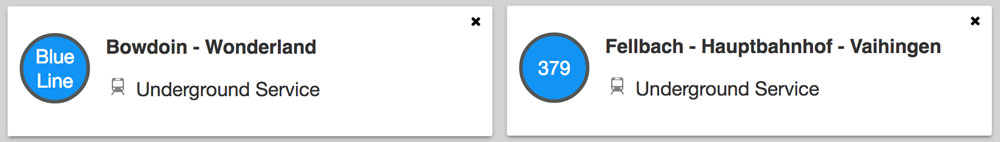
\includegraphics[width=\textwidth]{gtfs_differences.jpg}
        \caption{UI Element mit GTFS Informationen}
        \label{fig:gtfs_differences}
      \end{center}
    \end{figure}

    Links in der Abbildung ist die korrekte Bezeichnung der Route zu sehen nämlich \texttt{Blue Line}, wohingegen rechts nur eine numerische ID zu sehen ist, die nicht für den Nutzer vorgesehen und damit falsch ist. Damit die rechte Seite korrekt wäre müsste dort \texttt{U1} abgebildet sein. Die fehlende beziehungsweise nicht gegebene Übereinstimmung der beiden Feeds führt also zu Problemen bei der Darstellung die auch durch die Verwendung eines anderen Feldes wie zum Beispiel \texttt{route\_short\_name} nicht behoben werden können. 

    Dies ist nur ein Beispiel, bei dem Abweichungen in der Ausführung der Spezifikation eine Auswirkung auf die Programmierung haben. Aus diesem Grund ist im März 2017 auf \url{http://gtfs.org/} eine neue \texttt{Best-Practices} Sektion erschienen. Dabei handelt es sich um Empfehlungen an die Hersteller von GTFS Feeds, um eine Verwendung der Feeds möglichst zu vereinheitlichen. Würden sich alle Hersteller an solch eine striktere Implementierung der Spezifikation halten, müssten Programmierer weniger "`Edge Cases"'\footnotemark abfangen und Anwendungen würden in Qualität und Zuverlässigkeit noch besser werden.\\

    \footnotetext{Ein "`Edge Case"' ist ein Problem oder eine Situation, die nur bei einem extremen (maximalen oder minimalen) Betriebsparameter auftritt.}

    Ein weiteres Problem in GTFS ist das auslesen von Daten. GTFS lässt sich zwar sehr einfach in eine relationale Datenbank überführen, aber das Auslesen der Daten kann schnell sehr komplex werden, sodass die Geschwindigkeit für eine Webanwendung nicht mehr schnell ist. Bereits 1993 stellte \texttt{Jakob Nielsen} einen Richtwert für die responsive Wahrnehmung einer Webanwendung vor:

    \begin{quote}
      \textit{"`1.0 second is about the limit for the user's flow of thought to stay uninterrupted, even though the user will notice the delay. Normally, no special feedback is necessary during delays of more than 0.1 but less than 1.0 second, but the user does lose the feeling of operating directly on the data."'}\parencite{nielsen}
    \end{quote}

    Ob oder wie die Geschwindigkeit erreicht werden kann, soll hier nicht vertieft werden, denn zu diesem Thema habe ich bereits meine Bachelorarbeit gewidmet\parencite{lorer}.

    Damit eine Webanwendung aber überhaupt eine Chance hat, diese Geschwindigkeitsmarke zu erreichen, ist eine schnelle Antwortzeit des Backends sehr wichtig. Dabei sind Antwortzeiten Innerhalb von 1 bis 200 Millisekunden ein sehr guter Wert. Natürlich gilt: Je weniger umso besser. Diese Benchmark mit dem GTFS Format zu erreichen war eine der Hauptherausforderungen dieser Arbeit.\\

    Das GTFS Format hat den entscheidenden Nachteil, dass es eine hohe Komplexität aufweist, sobald Daten aus verschiedenen Tabellen benötigt werden. Für eine Live Visualisierung, sind Daten aus nahezu allen Tabellen relevant. Abbildung \ref{fig:gtfs_joined_tables} zeigt, welche davon benötigt - beziehungsweise nicht benötigt werden (grau).

    \begin{figure}[ht]
      \begin{center}
        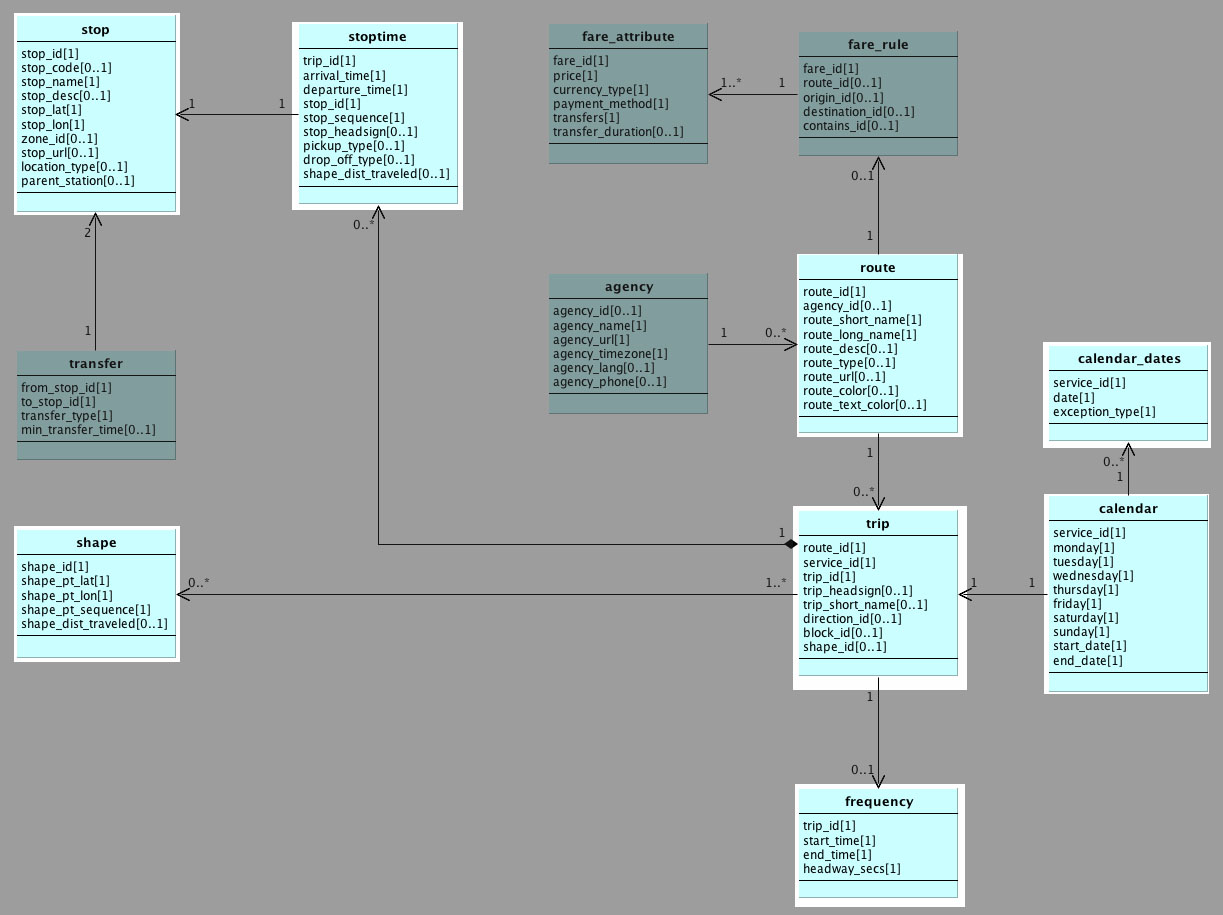
\includegraphics[width=\textwidth]{gtfs_joined_tables.jpg}
        \caption{Benötigte GTFS Tabellen\parencite{google_gtfs_reference}}
        \label{fig:gtfs_joined_tables}
      \end{center}
    \end{figure}

    Das UML Diagramm ist auf den ersten Blick relativ simpel zu verstehen und die Grundlagen der verschiedenen Relationen wurde bereits in Kapitel \ref{ssub:gtfs_fahrplandaten} beschrieben. Wo liegt also das Problem? In Worten ließe sich diese Datenbankabfrage mit folgendem Statement beschreiben: 

    \begin{quote}
      \label{query_statement}
      \textit{"`Gib uns alle aktiven Trips mit deren Linienverlauf, die am heutigen Tag aktiv sind und in einer Zeitspanne zwischen $t_a$ und $t_b$ liegen."'}
    \end{quote}

    Das große Problem dieses Satze liegt in der Zeitkomponente \textit{"`Trips die am heutigen Tag aktiv sind zwischen ..."'}. Die Trip Tabelle selbst (bezogen auf Abbildung \ref{fig:gtfs_joined_tables}), hat dies bezüglich keinerlei Informationen darüber. Auch die Calendar- und Calendar-Dates Tabelle beinhaltet nur Informationen, an welchem Datum ein Trip stattfindet, nicht aber um welche Uhrzeit. 

    Erst die Stoptime Tabelle ermöglicht es uns, eine Aussage zu treffen, wann ein Trip aktiv ist. Über die zwei Felder \texttt{arrival\_time} und \texttt{departure\_time} lässt sich sagen, zu welchem Zeitpunkt ein Vehicle an einer Station anhält. Die erste und letzte Station ($S_1$ und $S_n$) geben uns also einen zeitlichen Rahmen, in dem der Trip aktiv ist.
    Hierbei wird klar, dass allein die Beantwortung der Frage zur zeitlichen Komponente, bereits sehr viele Daten aus verschiedenen Tabellen benötigt. Die anderen Tabellen wie \texttt{shape}, \texttt{route}, \texttt{stop} und \texttt{frequency} würden für weitere Informationen wie Vehicle Farbe, Stop Position (Längen- und Breitengrad) oder die Polyline benötigt werden. Um an die Daten zu gelangen, müssen alle benötigten Tabellen mittels SQL \texttt{JOIN} miteinander verknüpft werden. Dies geschieht durch die Verbindung der einzelnen Reihen zweier Tabellen (TabelleA und TabelleB) gegen eine Verknüpfungsbedingung. Das Resultat ist eine neue Ergebnistabelle mit den Inhalten der kombinierten Reihen. Solche Verknüpfungen sind besonders dann Zeitintensiv, wenn eine große Menge an Daten (siehe Tabelle: \ref{table:table_metrics}) kombiniert werden. Die Metriken der Tabellen sind dabei wie folgt:

    \begin{longtable}{|>{\raggedright \arraybackslash}p{5.0cm}|>{\raggedright \arraybackslash}p{5.0cm}|>{\raggedright \arraybackslash}p{5.0cm}|}
    \caption{Tabellen Metriken} \label{table:table_metrics}\\
      \hline
      Tabellen Name & Anzahl Reihen\\
      \hline
      trips.txt & 71,000\\
      stop\_times.txt & 1,3000,000\\
      stops.txt & 7,900\\
      shapes.txt & 1,085,860\\
      \hline
    \end{longtable}
    
    Die für das oben genannte Statement \ref{query_statement} äquivalente SQL-Abfrage ist aufgrund seiner Länge (113 Zeilen Code) im Anhang unter Listing \ref{lst:get_active_trips_query} zu finden. Diese SQL Abfrage ist allerdings nicht Performant. Sollen alle Trips in einem Zeitraum von 1 - 15 Minuten gefunden werden, sind bereits Rechenzeiten entstanden, die aufgrund ihrer langen Laufzeit abgebrochen werden mussten. In mehreren Iterationen wurde versucht die SQL-Abfrage zu optimieren, was allerdings keine Verbesserung herbeiführte. Es sind zu viele JOIN Verknüpfungen und WHERE Bedingungen in dieser Abfrage, als dass sich eine Performante Lösung damit finden lässt. Es musste ein neuer Ansatz gefunden werden um Abfragezeiten erheblich zu verringern.
  % subsubsection freiräume_in_der_gestaltung_von_gtfs (end)